\textbf{COLUNI 2025 -- Questão 30}\par\medskip Uma nova espécie de morcego foi descoberta por pesquisadores brasileiros e mexicanos, no sudoeste do México. Medindo apenas 5 cm de comprimento e pesando cerca de 10 gramas, ela é uma das menores de seu grupo, que possui mais de 30 espécies nas Américas. Os pesquisadores coletaram três indivíduos, dois machos e uma fêmea, e os compararam com outros morcegos do mesmo grupo usando análises morfológicas e genéticas.

% COLUNI-AUTO-FIGURES-BEGIN
\begin{figure}[htbp]
\centering
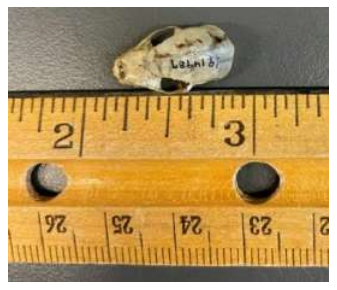
\includegraphics[width=0.28\linewidth]{static/simulados/coluni/figuras/2025/questao-30/figura-1.png}
\end{figure}
% COLUNI-AUTO-FIGURES-END
\noindent Disponível em: https://theconversation.com/uma-das-menores-especies-de-morcegos-frugivoros-do-mundo-e-descoberta-por-cientistas-brasileiros-e-mexicanos. Acesso em: 05 Ago. 2024. Adaptado.

Considerando o sistema de classificação dos seres vivos e as regras de nomenclatura para os nomes científicos, assinale a alternativa que indica CORRETAMENTE a classe e o nome da espécie identificada:
\begin{enumerate}
\item Classe Mammalia, \textit{Vampyressa villai}.
\item Classe Aves, \textit{vampyressa Villai}.
\item Classe Mammalia, \textit{vampyressa Villai}.
\item Classe Aves, \textit{VAMPYRESSA VILLAI}.
\end{enumerate}
